\documentclass[problem]{mcs}

\begin{pcomments}
  \pcomment{FP_AND_circuit}
  \pcomment{ARM 9/22/15}
  \pcomment{from: S17.cp2w, F15.midterm1}
  \pcomment{overlaps FP_AND_circuit_shorter}
  \pcomment{COMBINE WITH FP_AND_circuit_shorter, have induction
    version back ref to avoid repeat figures.}
\end{pcomments}

\pkeywords{
  circuit
  digital
  binary
  serial
  tree
  latency
}

%%%%%%%%%%%%%%%%%%%%%%%%%%%%%%%%%%%%%%%%%%%%%%%%%%%%%%%%%%%%%%%%%%%%%
% Problem starts here
%%%%%%%%%%%%%%%%%%%%%%%%%%%%%%%%%%%%%%%%%%%%%%%%%%%%%%%%%%%%%%%%%%%%%

\begin{problem}
  An $n$-bit $\QAND$-circuit has 0-1 valued inputs $a_0,a_1,\dots,a_{n-1}$ and
  one output $c$ whose value will be 
   \[
   c = a_0 \QAND a_1 \QAND \cdots \QAND a_{n-1}.
   \]

  There are various ways to design an $n$-bit $\QAND$-circuit.  A
  \emph{serial} design is simply a series of $\QAND$-gates, each with
  one input being a circuit input $a_i$ and the other input being the
  output of the previous gate as shown in Figure~\ref{fig:serial-AND}.

\begin{figure}

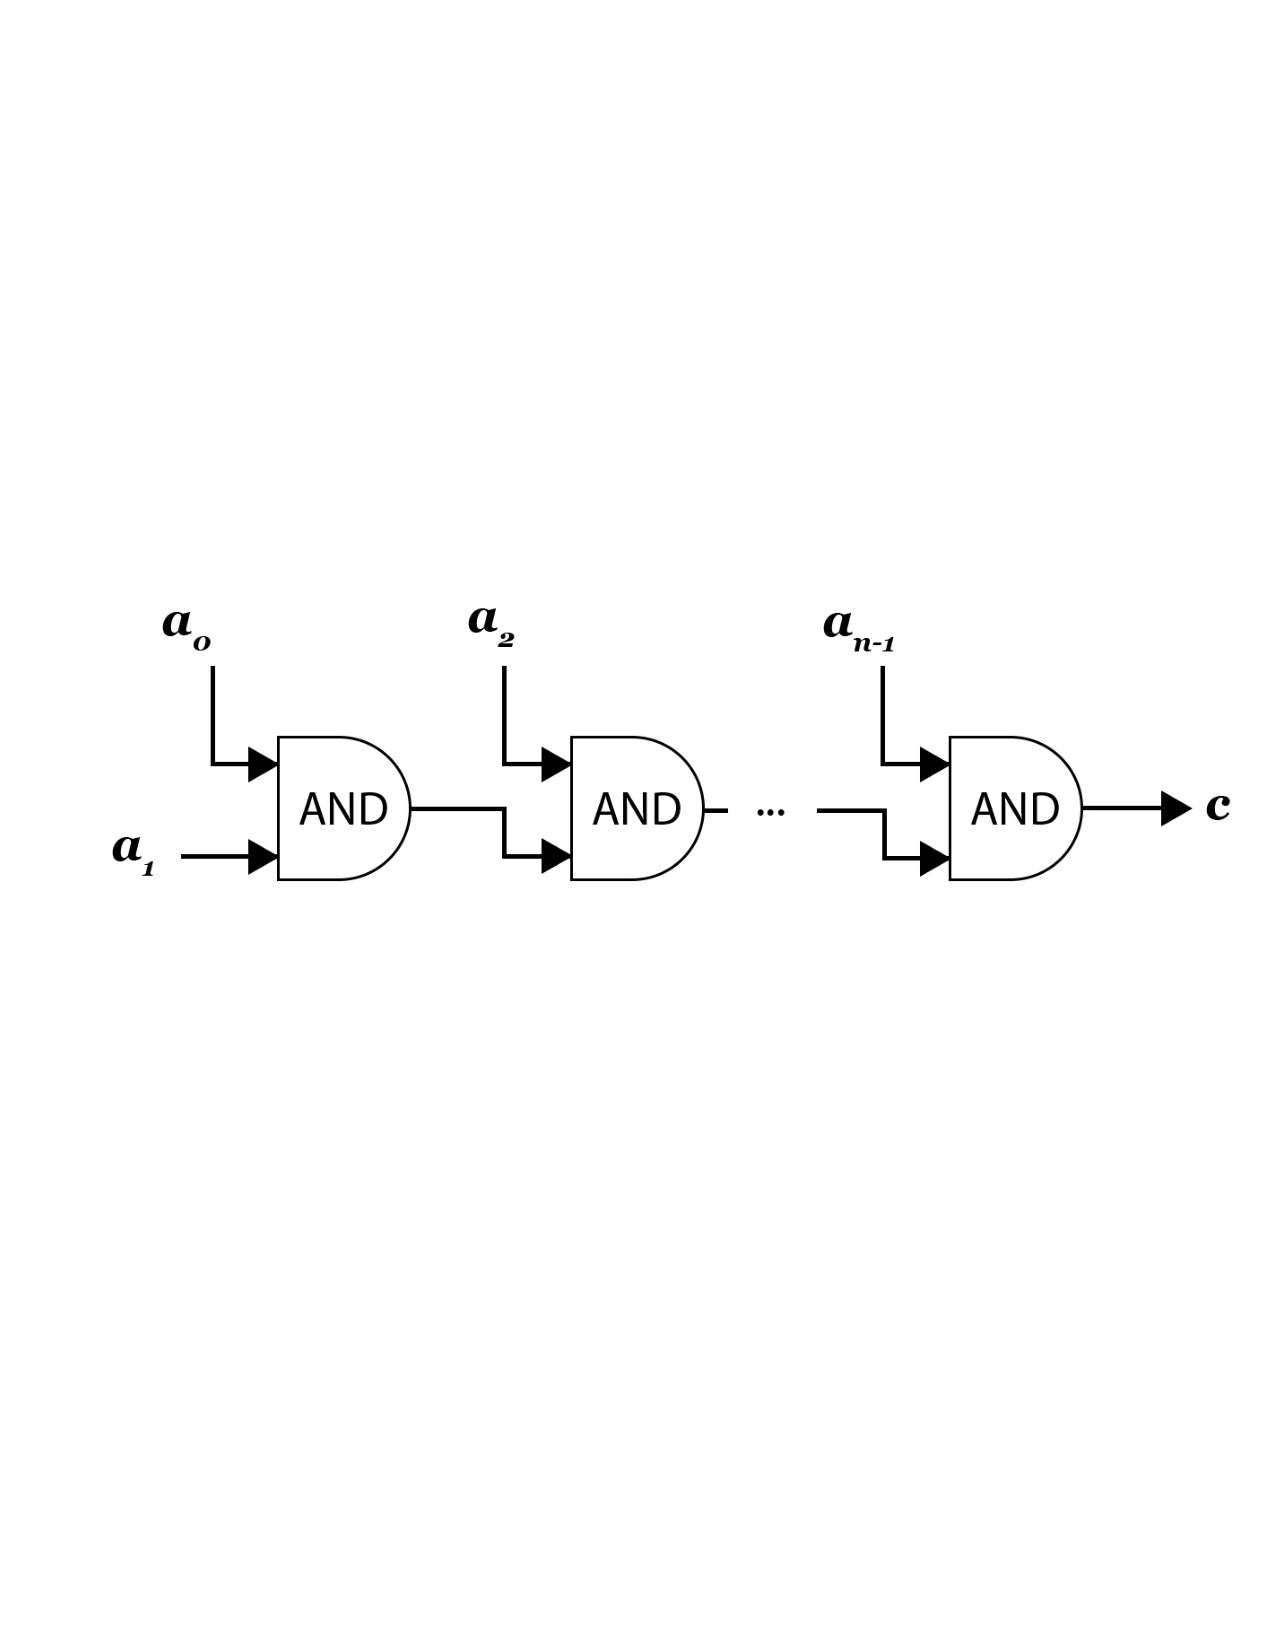
\includegraphics[width=4in]{AND_serial}

\caption{A serial $\QAND$-circuit.}
\label{fig:serial-AND}
\end{figure}

  We can also use a \emph{tree} design.  A 1-bit tree design is just a
  wire, that is $c \eqdef a_1$.  Assuming for simplicity that $n$ is a
  power of two, an $n$-input tree circuit for $n>1$ simply consists of
  two $n/2$-input tree circuits whose outputs are $\QAND$'d to produce
  output $c$, as in Figure~\ref{fig:AND-tree-n}.  For example, a
  4-bit tree design circut is shown in Figure~\ref{fig:AND-tree-4}.

\begin{figure}

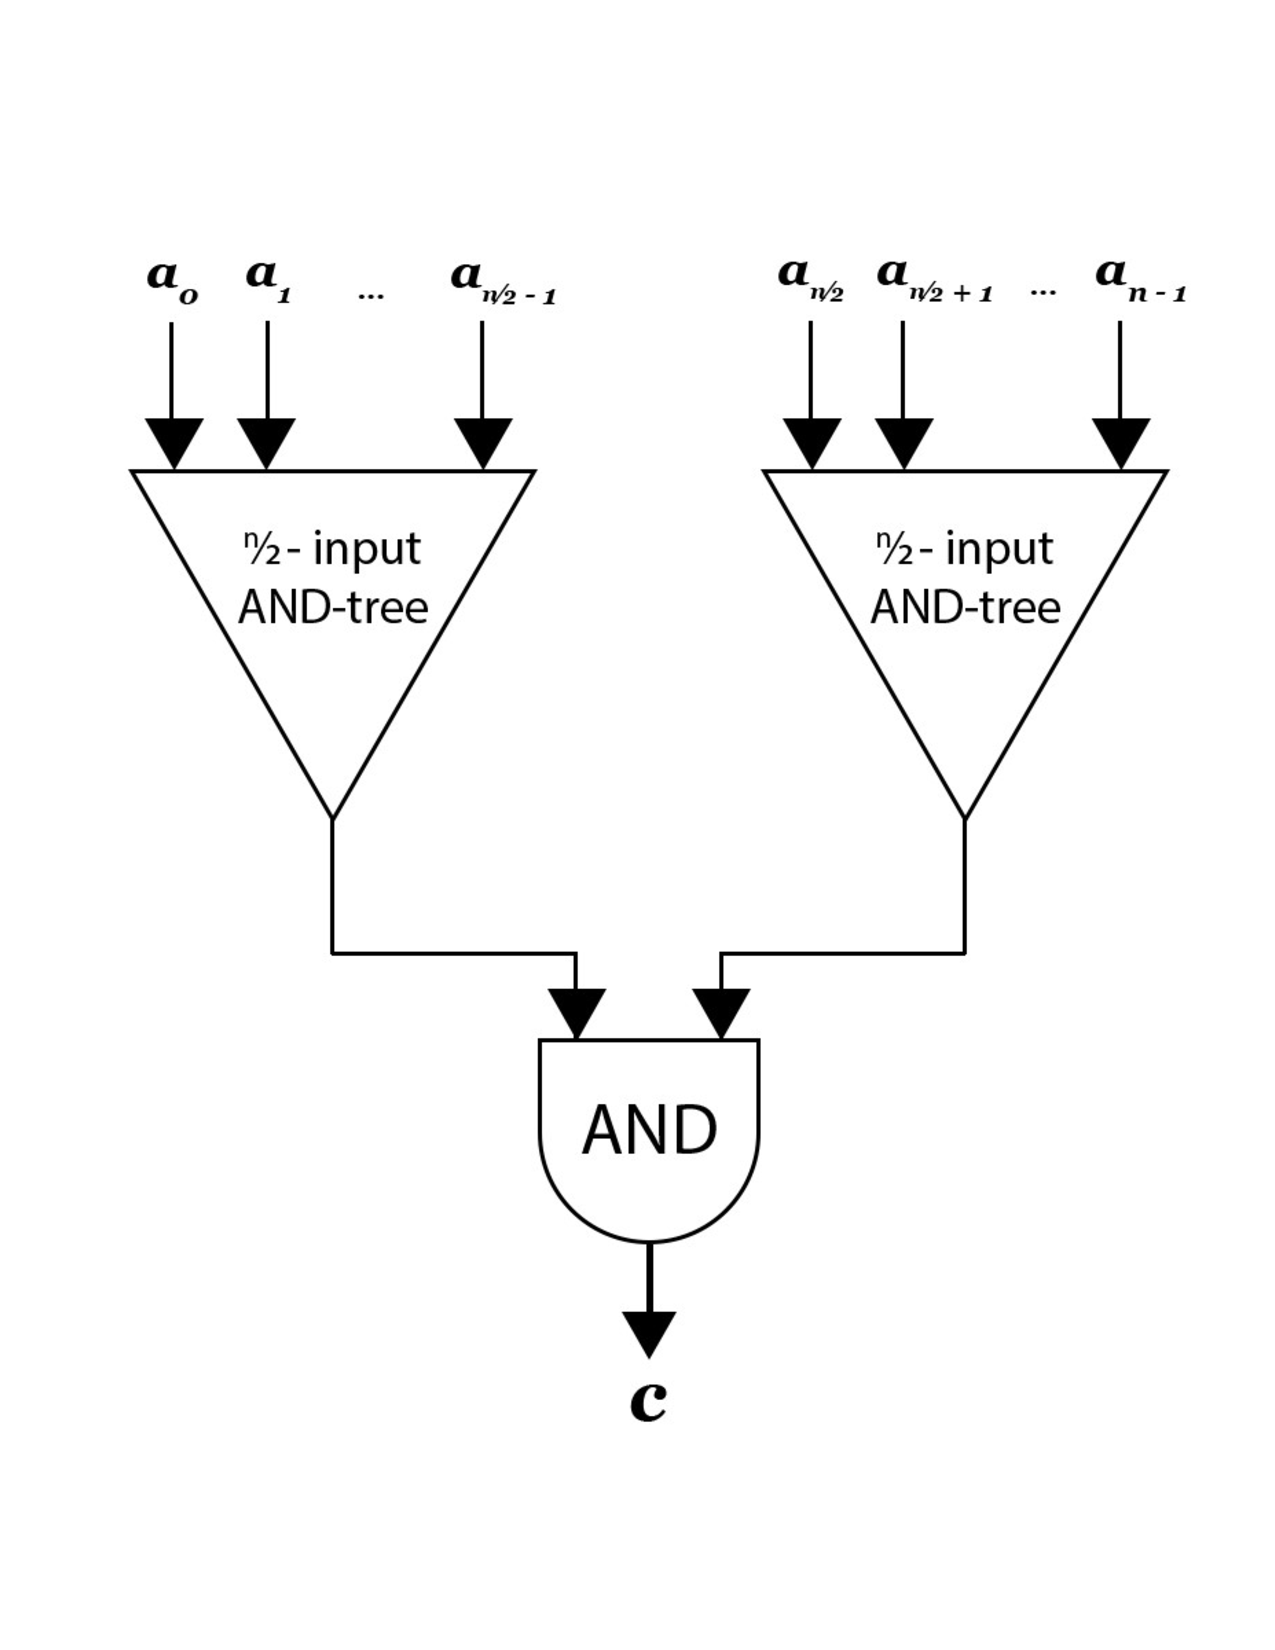
\includegraphics[height=4in]{AND_tree_recursive}

\caption{An $n$-bit $\QAND$-tree circuit.}
\label{fig:AND-tree-n}
\end{figure}

\begin{figure}

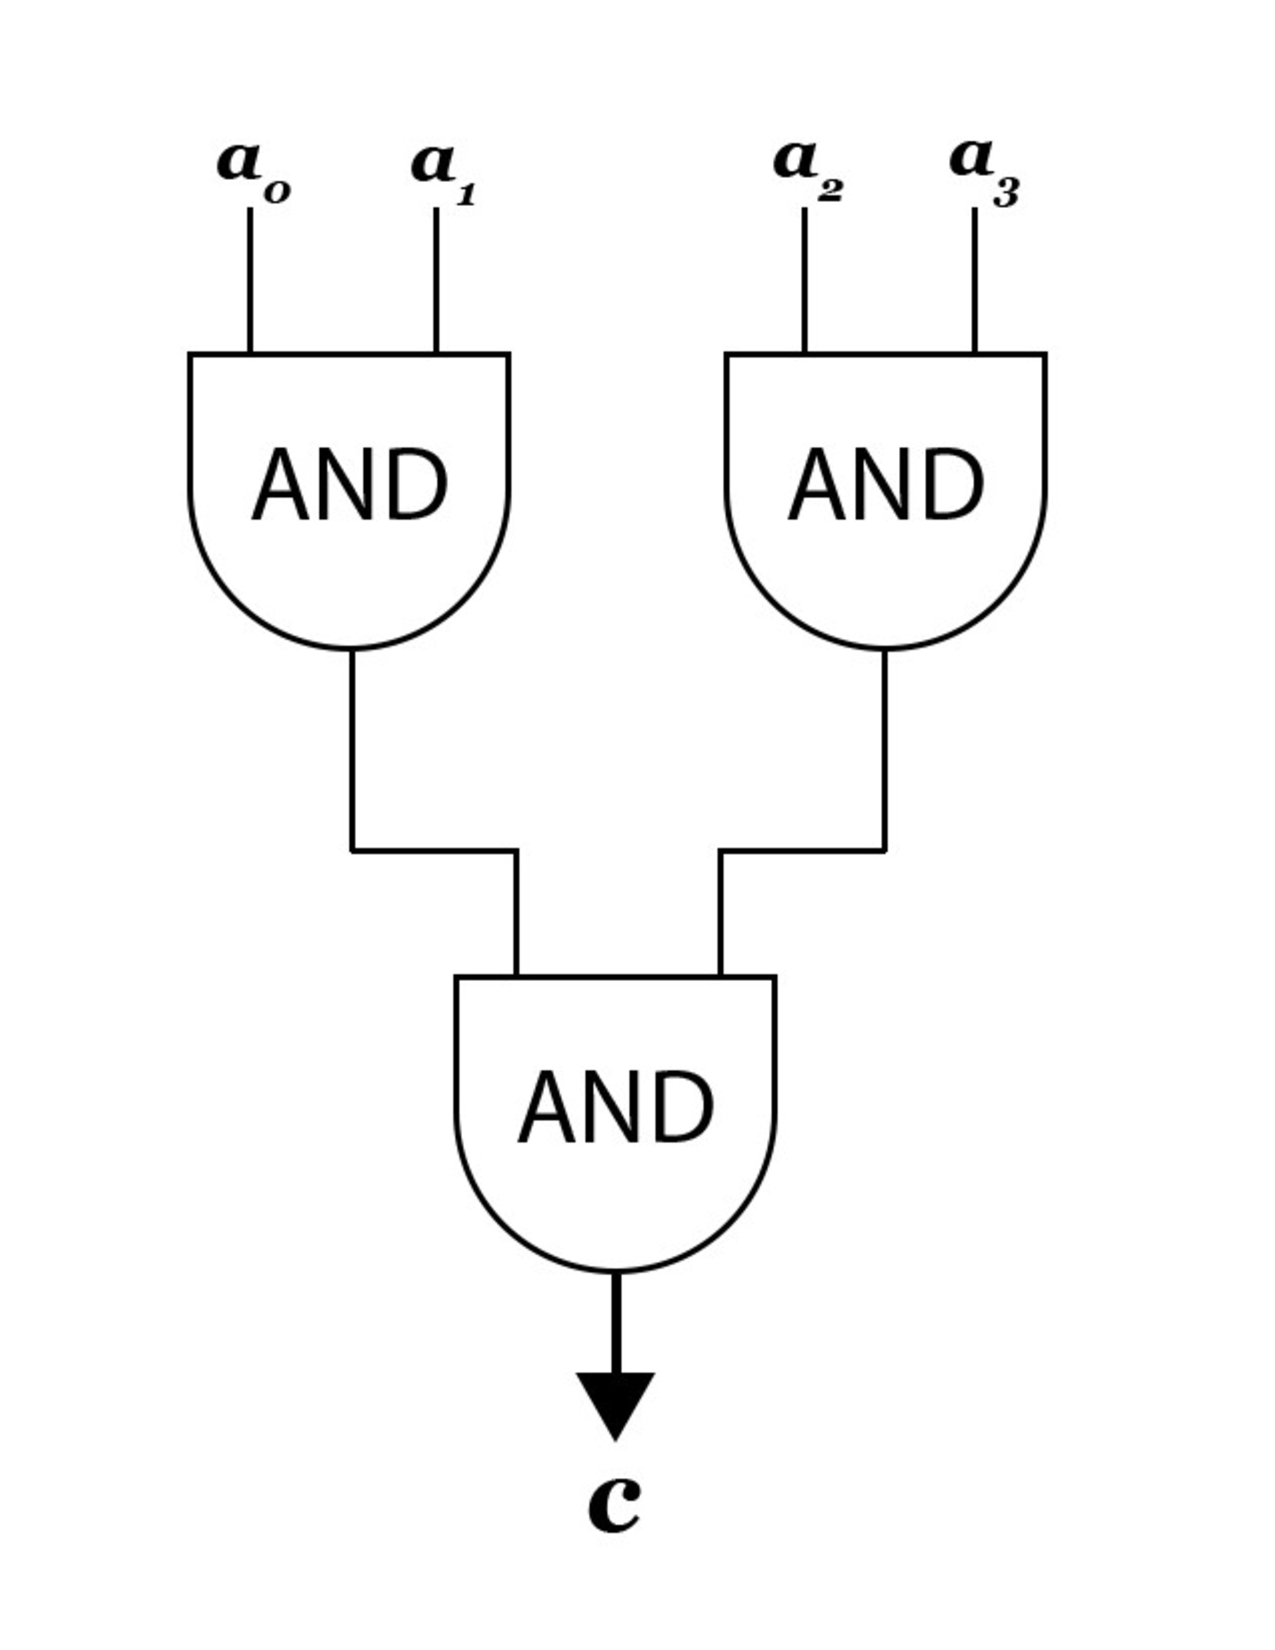
\includegraphics[height=2.0in]{AND_tree_4}

\caption{A $4$-bit $\QAND$-tree circuit.}
\label{fig:AND-tree-4}
\end{figure}

\bparts

\ppart How many $\QAND$-gates are in the $n$-input serial
circuit?\examrule[0.7in]

\begin{solution}
$n-1$.
\end{solution}

\ppart The ``speed'' or \emph{latency} of a circuit is the largest
number of gates on any path from an input to an output.  Briefly
explain why the tree circuit is \emph{exponentially faster} than the
serial circuit.

\examspace[2in]

\begin{solution}
For the $n$-input serial circuit, the longest such path is from $a_1$
to $c$, and it has $n-1$ $\QAND$-gates.  For a one-input tree-circuit,
there are no gates on the path from input to output.  For an $n\geq
2$-input tree circuit, the number of gates on every path from an input
to output is one plus the length of a path from an $n/2$-input tree
circuit to its output.  That is the path length increases by one when
the number of inputs doubles.  This implies that the number of gates
on an input to output path in an $n$-input tree-circuit is $\log_2 n$,
which is exponentially smaller than $n$.
\end{solution}

\ppart Assume $n$ is a power of two. Prove \inhandout{using the Well
  Ordering Principle} that the $n$-input tree circuit has $n-1$
$\QAND$-gates.
 
\examspace[5in]

\begin{solution}
Suppose some $n$-bit tree circuit had a different number of
$\QAND$-gates.  By WOP, there is a least $m$ such that $m$ is a power
of two and the $m$-bit tree circuit does not have $m-1$ gates.

When $n=1$, then $n-1$ is zero.  Since the 1-bit tree circuit has no
gates, $n-1$ is the correct formula when $n=1$, so $m$ must be $>1$.
Also, $m$ is a power of two, so it must be divisible by 2.  So $m/2$
is a smaller power of 2, and since $m$ is minimum number for which the
$n-1$ count fails, an $m/2$-input tree circuit must have $m/2-1$
$\QAND$-gates.  But since the $m$-input tree is made out of two
$m/2$-input trees plus one $\QAND$-gate, it has $(m/2-1)+(m/2-1)+1 =
m-1$ $\QAND$-gates, contradicting the assumption that the $m$-input
tree has a different number of gates.  This contradiction implies that
the $n$-bit tree circuit has $n-1$ gates for every $n$ that is a power
of 2.
\end{solution}
\eparts
\end{problem}

%%%%%%%%%%%%%%%%%%%%%%%%%%%%%%%%%%%%%%%%%%%%%%%%%%%%%%%%%%%%%%%%%%%%%
% Problem ends here
%%%%%%%%%%%%%%%%%%%%%%%%%%%%%%%%%%%%%%%%%%%%%%%%%%%%%%%%%%%%%%%%%%%%%

\endinput

\iffalse
Serial is described by
   the formulas:
   \begin{align*}
     c_1     & \eqdef a_1 \QAND\ a_0\\
     c_2     & \eqdef a_2 \QAND\ c_1\\
     c_3     & \eqdef a_3 \QAND\ c_2\\
             & \vdots\\
     c_{n-1}  & \eqdef a_{n-1} \QAND\ c_{n-2}\\
     c       & \eqdef c_{n-1}.
\end{align*}


  The tree design is
  described by formulas involving binary variables $t_y$ where
  $y$ ranges over binary strings of length $\leq k$.  Any such
  positive length string $y$ is a binary representation of a
  nonnegative integer $\binnum{y}$ less than $n$.  For example,
\[
  \binnumt{00001} = 1, \quad \binnumt{010} = 2, \quad \binnumt{11} =
  3, \binnumt{110} = 6, \quad \binnumt{0111} = 7.
\]

  We begin by defining
  \[
  t_y \eqdef a_{\binnum{y}} \text{   (for $y$ of length $k$)}.
  \]
  For $y$ of length less than $k$, define
  \[
   t_{y} \eqdef t_{y\mtt{0}} \QAND\ t_{y\mtt{1}}
   \]
   So
  \begin{align*}
   t_{\emptystring} & \eqdef t_{\mtt{0}} \QAND\ t_{\mtt{1}}\\
   t_{0} & \eqdef t_{\mtt{00}} \QAND\ t_{\mtt{01}}\\
   t_{1} & \eqdef t_{\mtt{10}} \QAND\ t_{\mtt{11}}\\
   t_{00} & \eqdef t_{\mtt{000}} \QAND\ t_{\mtt{001}}\\
        & \vdots
  \end{align*}
  Finally, the output $c$ is
  \[
  c  \eqdef t_{\emptystring}.
   \]
\fi
